\documentclass[Chap2bmain.tex]{subfiles}

% Load any packages needed for this document
\begin{document}
\newpage
%--------------------- %

\section{Multivariate}
\subsection{Mahalanobis Distance }

The Mahalanobis Distance is a descriptive statistic that provides a relative measure of a data point's distance (residual) from a common point. It is a unitless measure introduced by P. C. Mahalanobis in 1936.[1] The Mahalanobis distance is used to identify and gauge similarity of an unknown sample set to a known one. It differs from Euclidean distance in that it takes into account the correlations of the data set and is scale-invariant. In other words, it has a multivariate effect size.

\section{Bartko's Ellipse}
As a complement to the Bland-Altman plot, \textit{Bartko} proposes
the use of a bivariate confidence ellipse, constructed for a
predetermined level. \textit{AltmanEllipse} provides the relevant calculations for the
ellipse. This ellipse is intended as a visual
guidelines for the scatter plot, for detecting outliers and to
assess the within- and between-subject variances.

The minor axis relates to the between subject variability, whereas
the major axis relates to the error mean square, with the ellipse
depicting the size of both relative to each other.
Consequently Bartko's ellipse provides a visual aid to determining the
relationship between variances. If $\mbox{var}(a)$ is greater than $\mbox{var}(d)$, the orientation of the ellipse is horizontal. Conversely if $\mbox{var}(a)$ is less than $\mbox{var}(d)$, the orientation of the ellipse is vertical.


%(Furthermore \citet{Bartko}
%proposes formal testing procedures, that shall be discussed in due
%course.)

The Bland-Altman plot for the Grubbs data, complemented by Bartko's ellipse, is depicted in Figure 1.7.
The fourth observation is shown to be outside the bounds of the ellipse, indicating that it is a potential outlier.


%\begin{figure}[h!]
%  % Requires \usepackage{graphicx}
%  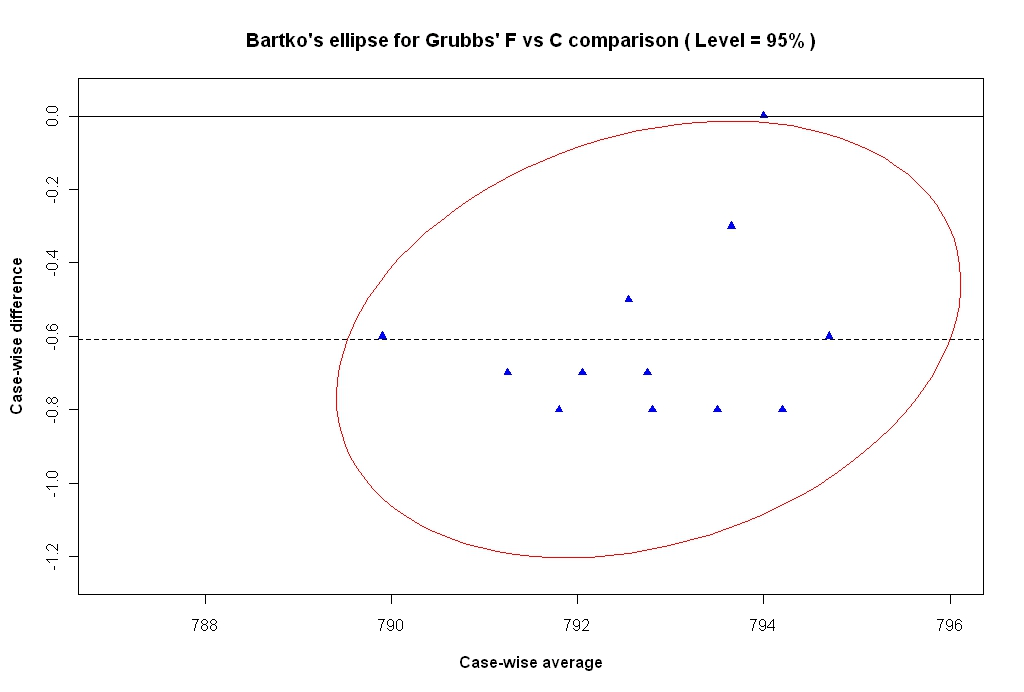
\includegraphics[width=130mm]{GrubbsBartko.jpeg}
%  \caption{Bartko's Ellipse For Grubbs' Data.}\label{GrubbsBartko}
%\end{figure}

The limitations of using bivariate approaches to outlier detection
in the Bland-Altman plot can demonstrated using Bartko's ellipse.
A covariate is added to the `F vs C' comparison that has a
difference value equal to the inter-method bias, and an average
value that markedly deviates from the rest of the average values
in the comparison, i.e. 786. Table 1.8 depicts a $95\%$ confidence
ellipse for this manipulated data set. By inspection of the
confidence interval, a conclusion would be reached that this extra
covariate is an outlier, in spite of the fact that this
observation is wholly consistent with the conclusion of the
Bland-Altman plot.

%\begin{figure}[h!]
%  % Requires \usepackage{graphicx}
%  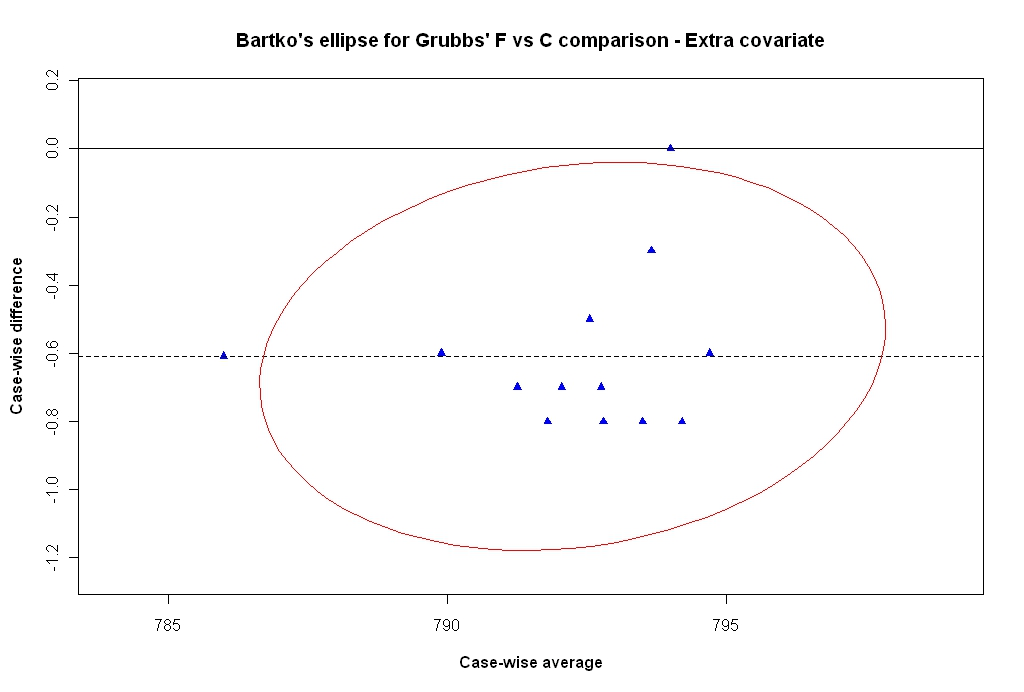
\includegraphics[width=130mm]{GrubbsBartko2.jpeg}
%  \caption{Bartko's Ellipse For Grubbs' Data, with an extra covariate.}\label{GrubbsBartko2}
%\end{figure}


Importantly, outlier classification must be informed by the logic of the
data's formulation. In the Bland-Altman plot, the horizontal displacement of any
observation is supported by two independent measurements. Any
observation should not be considered an outlier on the basis of a
noticeable horizontal displacement from the main cluster, as in
the case with the extra covariate. Conversely, the fourth
observation, from the original data set, should be considered an
outlier, as it has a noticeable vertical displacement from the
rest of the observations.

%Grubbs' test is a statistical test used for detecting outliers in a
%univariate data set that is assumed to be normally distributed.

%\citet{Grubbs} defined an outlier as a co-variate that appears to
%deviate markedly from other members of the sample in which it
%occurs.

In classifying whether a observation from a univariate data set is
an outlier, many formal tests are available, such as the Grubbs test for outliers. In assessing
whether a covariate in a Bland-Altman plot is an outlier, this
test is useful when applied to the case-wise difference values treated as a
univariate data set. The null hypothesis of the Grubbs test procedure is the absence
of any outliers in the data set. Conversely, the alternative hypotheses is that there is at least one outlier
present.

The test statistic for the Grubbs test ($G$) is the largest
absolute deviation from the sample mean divided by the standard
deviation of the differences,
\[
G =  \displaystyle\max_{i=1,\ldots, n}\frac{\left \vert d_i -
\bar{d}\right\vert}{S_{d}}.
\]

For the `F vs C' comparison it is the fourth observation gives
rise to the test statistic, $G = 3.64$. The critical value is
calculated using Student's $t$ distribution and the sample size,
\[
U = \frac{n-1}{\sqrt{n}} \sqrt{\frac{t_{\alpha/(2n),n-2}^2}{n - 2
+ t_{\alpha/(2n),n-2}^2}}.
\]
For this test $U = 0.75$. The conclusion of this test is that the fourth observation in the `F vs C' comparison is an outlier, with $p-$value = 0.003, according with the previous result using Bartko's ellipse.

\end{document}
